% --------------------------------------------------------------
% This is all preamble stuff that you don't have to worry about.
% Head down to where it says "Start here"
% --------------------------------------------------------------
 
\documentclass[twocolumn]{article}
 
 
\usepackage[T1]{fontenc}
\usepackage[margin=1in]{geometry} 
\usepackage{amsmath,amsthm,amssymb}
\usepackage{graphicx}
\usepackage{cite}
\usepackage{amsmath}
\graphicspath{ {../media/} } 

\newcommand{\N}{\mathbb{N}}
\newcommand{\Z}{\mathbb{Z}}
\newcommand\indep{\protect\mathpalette{\protect\independenT}{\perp}}
\def\independenT#1#2{\mathrel{\rlap{$#1#2$}\mkern2mu{#1#2}}}

\newenvironment{theorem}[2][Theorem]{\begin{trivlist}
\item[\hskip \labelsep {\bfseries #1}\hskip \labelsep {\bfseries #2.}]}{\end{trivlist}}
\newenvironment{lemma}[2][Lemma]{\begin{trivlist}
\item[\hskip \labelsep {\bfseries #1}\hskip \labelsep {\bfseries #2.}]}{\end{trivlist}}
\newenvironment{exercise}[2][Exercise]{\begin{trivlist}
\item[\hskip \labelsep {\bfseries #1}\hskip \labelsep {\bfseries #2.}]}{\end{trivlist}}
\newenvironment{reflection}[2][Reflection]{\begin{trivlist}
\item[\hskip \labelsep {\bfseries #1}\hskip \labelsep {\bfseries #2.}]}{\end{trivlist}}
\newenvironment{proposition}[2][Proposition]{\begin{trivlist}
\item[\hskip \labelsep {\bfseries #1}\hskip \labelsep {\bfseries #2.}]}{\end{trivlist}}
\newenvironment{corollary}[2][Corollary]{\begin{trivlist}
\item[\hskip \labelsep {\bfseries #1}\hskip \labelsep {\bfseries #2.}]}{\end{trivlist}}
 
\begin{document}
 
% --------------------------------------------------------------
%                         Start here
% --------------------------------------------------------------
 
%\renewcommand{\qedsymbol}{\filledbox}
 
\title{\textbf{\boldmath$m^3GAN$: Multi-Modal Matching with Generative Adversarial Networks}}
\author{\textbf{Ntavelis, Evangelos}\\ %replace with your name
Master of Artificial Intelligence \\
KULeuven \\
\texttt{evangelos.ntavelis@student.kuleuven.be}
\and
\textbf{Collell, Guillem}
\\
Computer Science Department\\
KULeuven\\
\texttt{gcollell@kuleuven.be}
\and
\textbf{Moens, Marie-Francine}\\
Computer Science Department\\
KULeuven\\
\texttt{sien.moens@cs.kuleuven.be}
\date{}
} %if necessary, replace with your course title
 
\maketitle

\textbf{
  \textit{Abstract--} Humans' understanding of the world is grounded on all of our senses.
Accordingly, being able to create a representation that incorporates information of more than one modality has many applications in a great variety of Natural Language Processing and Computer Vision Tasks.
  Recently, Generative Adversarial Networks have been proposed to tackle the problem of cross-modal retrieval.
  Yet, these works are limited to the domain of representations.
  We propose the \boldmath$m^3GAN$ architecture as a way to create representations by simultaneously training a network to caption images and generate images given a caption.
  To train our network we use two pathways from one modality to the other.
 Each modality's input is encoded in a representation vector which will be then decoded to an output of the other modality, and two discriminator networks will test the quality of the produced results.
 At the same time, we use the encoder networks previously used on the input data to create a vector representation of the produced outputs.
 This way we can also measure both an inter- and an intra-modal reconstruction loss at the representation level.   
 The resulted representations are then tested on a cross-modal retrieval task.
}
\section{Introduction}

There is evidence that the nature of human memory is reconstructive \cite{ACS, onInt}. That means that our neural system breaks down the stimuli it receives from the outside world into an internal representation and it recreates it when the need arises. Moreover, Barsalou\cite{doi:10.1146/annurev.psych.59.103006.093639} argues that ground cognition draws upon the senses. It's normal, thus, to aim to computationally recreate this multi-modal decomposition, coding and composition procedure.

In the previous years we can observe a lot of approaches tackling this problem using auto-encoders, both combining audio and visual features \cite{conf/icml/NgiamKKNLN11} and visual and text features \cite{silberer2014learning}. The encoders were fed with pre-learned features independently for both modalities, which were then combined \textit{a posteriori}. 

More recently, a generative family of models, Generative Adversarial Networks, have gained popularity. Among other things, they were used as an alternative method to design multi-modal embeddings in video hyperlinking with promising results\cite{DBLP:journals/corr/VukoticRG17}.

Here, we propose an architecture that tries to match representations created from one modality with the corresponding ones of an other. The main idea is that given one modality we try to create the other. So, given an image we are trying to create the text, or \textit{caption}, that describes its contents, while at the same time we are trying to generate an image given a text description. The discriminator networks will ensure that the produced results are realistic and the imposed representation reconstruction losses will establish that our representations our networks produce are able to meaningfully incorporate information.

The paper is organized in the following way. The next session describes a plethora of papers related to the task at hand. Related work and background are discussed in the second section. We later analyze the notation and architecture of our model. Then, we report on the experimental results before concluding with the last section.


\section{Related Work and Background}

Peng et al 2017 \cite{DBLP:journals/corr/abs-1710-05106} and Wang et al \cite{acmr} seem to follow a similar approach to utilize an adversarial setting \cite{2014arXiv1406.2661G} for \textit{Cross-Modal Representation Learning}.
In both articles we observe the usage of initial representations derived from a unimodal setting:

\begin{itemize}
  \item{Visual Embedding:} 4,096 dimension feature vector from the fc7 layer of a VGG-Net trained on ImageNet for both cases
  \item{Word Embeddings:} 
    \begin{itemize}
      \item $n \times x$ matrix, with n the number of words and k the number of Word2Vec Features\cite{DBLP:journals/corr/MikolovSCCD13}
      \item Bag of Words vector with TF-IDF weighting
    \end{itemize}
\end{itemize}


They both use fully connected layers to arrive to a common representation and use discriminators inter-modally and intra-modally. Yet the approaches differ in their implementations and also the acmr method uses a label predictor as an additional discriminator network.


Since the introduction of Generative Adversarial Networks in 2014 by Ian Goodfellow\cite{2014arXiv1406.2661G} the architecture has produced a lot of promising results in a variety of tasks. Especially after the introduction of DCGANs we observed significant results in unsupervised representation learning\cite{DBLP:journals/corr/RadfordMC15}. The performance of GANs was later improved by the stabilization of their training \cite{DBLP:journals/corr/RothLNH17, Arjovsky2017Jan}. 

These networks have also been used in tasks than combine language and vision. Reed et. al\cite{reed2016generative} introduced an architecture to synthesize images given a text description. Using stacked layers of GANs and, additionally in their last work, incorporating attention Tao Xu, Han Zhang et al.\cite{han2017stackgan,DBLP:journals/corr/abs-1710-10916,DBLP:journals/corr/abs-1711-10485} created realistic images. Moreover, on the image captioning task, following the \textit{Show, Attend and Tell} model \cite{DBLP:journals/corr/XuBKCCSZB15} Chen et al. created the \textit{Show, Adapt and Tell} model for cross-domain image captioning \cite{chen2017show}.

GANs have produced interesting results both in image translation\cite{DBLP:journals/corr/KimCKLK17, DBLP:journals/corr/LiuBK17}  and language generation tasks\cite{DBLP:journals/corr/RajeswarSDPC17}. 

By applying an approach similar to Disco-GANs\cite{DBLP:journals/corr/KimCKLK17} on a multi-modal setting we will train a network for a cross-modal retrieval task. Specifically, we measure the cross-modal retrieval performance in terms of mAP on the tested dataset (e.g. MSCOCO\cite{dblp:journals/corr/linmbhprdz14}). 

\section{Proposed Method}

Our method, as shown in Figure \ref{arch} is composed by two pathways. We are using the dataset MSCOCO and for each image in our training set we have five captions. Our goal is to simultaneously train the network to produce descriptions of images given the images and generate images given a description. This is achieved by utilizing six sub networks in total:
\begin{itemize}
  \item \textbf{Image Encoder:} A \textit{Convolutional Neural Network} is used to map the image to the common representation space
  \item \textbf{Text Decoder:} The text generator of our first GAN is a \textit{Long-Short Term Memory Network} that transforms the representation vector to a word embeddings sequence
  \item \textbf{Text Encoder:} A \textit{bidirectional Long-Short Term Memory Network} that projects a sentence(caption) to the representation domain
  \item \textbf{Image Decoder} The image generator of our second GAN is \textit{Deconvolutional Neural Network} that has as input the representation vector concatenated with a noise vector and outputs an image
  \item \textbf{Image Discriminator:} A \textit{Convolutional Neural Network} that tries to tell generated images apart from the ones present on the training data
  \item \textbf{Text Discriminator:} A \textit{Long-Short Term Memory Network} that determines the probability that its input's lingual sequence is fabricated 

\end{itemize}

\begin{figure*}
  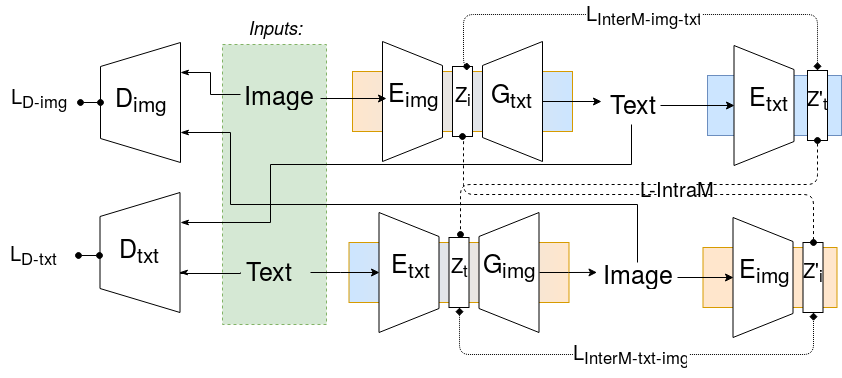
\includegraphics[width=\textwidth]{media/mmmGanwide}
  \caption{$m^3Gan$ Architecture.}
  \label{arch}
\end{figure*}


\subsection{Data Preparation}

All the images in the MSCOCO dataset are resized to dimensions of 256x256. All words of frequency less than 4 are omitted from the vocabulary, the rest are tokenized. Based on the resulting vocabulary we turn the captions into sequences of GloVe embeddings\cite{pennington2014glove} with dimension of 100, before feeding them to the network.

\subsection{Networks Pre-training}

\begin{figure}
  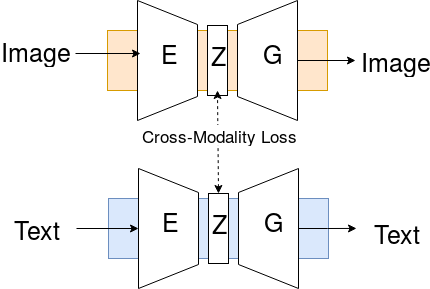
\includegraphics[width=0.5\textwidth]{media/pretraining}
  \caption{Pre-training of our networks.}
  \label{pretrain}
\end{figure}


Before training the architecture on the cross-modal setting, we train the encoder/decoder networks in a auto-encoder fashion, as show in Figure \ref{pretrain}.
All our schemes share the same color coding. The light orange background denotes that an \textit{encoder}(or \textit{decoder}) has \textit{input}(or \textit{output}) of visual data. The light blue background is used for text inputs and outputs.

The encoder networks map from a unimodal to the multi-modal domain and the decoders vice-versa. Their task has the same nature both in the case they are used as parts of an auto-encoder and as parts of a inter-modal translation network. Yet translating back to the same modality is an easier task with well defined objective functions. For the case of image translation we can use various distance functions such as MSE, cosine distance, and hinge-loss\cite{DBLP:journals/corr/KimCKLK17}. For the textual reconstruction the cross-entropy between the input and its reconstruction \cite{oshri2016there}.

The two auto-encoders are paired during the training. For each image iteration on the visual network we train on its five captions on the language model. During the process we impose a cross-modal loss between the intermediate representations, denoted as $Z$ in Figure \ref{pretrain}. This auxiliary loss can also be MSE, cosine distance or \textit{the squared difference of the dot product of the two representation vectors and one}. An additional parameter $\alpha$ can be used to determine the percentage of the overlapping we want to take into account between the two vectors.\footnote{The idea is that the representation hyperplanes of the two modalities are not purely identical, so we only consider that they share a subset of their dimensions. The remaining dimensions are descriptive of features unique to the particular modality.}

The imposed loss function makes the two vectors represent features that are activated by the pictures and their corresponding captions to share similar positions in the vector. This will prove useful when we will swap the decoder networks of the two encoder-decoder pairs as the background colors denote on figures \ref{pretrain} and \ref{arch}.  

At this point we already have representations whose performance we can gauge on a cross-modal retrieval task.

\subsection{Our Model}

Hereby, we describe the notation and our architecture. When \boldmath$i$ is used, the referenced variable is in the image domain, in case of \boldmath$t$ in the lingual domain and we use \boldmath$z$ for a vector in the representation space. 

The \textit{Image Encoder} \boldmath$E_{img}$ takes an image of dimensions 256x256x3 and transforms it to a vector in the common multi-modal space of dimension 300. This vector is then used as input to the \textit{Text Decoder}(Text Generator) \boldmath$G_{txt}$ who transforms it on a sequence of GloVe embeddings.

\[ z_i = E_{img}(i) \]

\[ t' = G_{txt}\circ E_{img}(i) = G_{txt}(z_i) \]

In parallel, the \textit{Text Encoder}(Text Generator) \boldmath$E_{img}$ takes the caption transformed to a sequence of GloVe embeddings as an input. The output is also a vector of 300 elements which is then fed to the \textit{Image Decoder}(Image Generator) \boldmath$G_{txt}$ concatenated with a vector of noise. 

\[ z_t = E_{txt}(t) \]

\[ i' = G_{img}\circ E_{txt}(t) = G_{img}(z_t) \]


Each of the Generators produces an output that is then fed to the two discriminator networks, the \textit{Image Discriminator} \boldmath$D_{img}$ and the \textit{Text Discriminator} \boldmath$D_{txt}$. Using the results of those two networks we can compute our Generative Adversarial Losses and the GAN discriminator losses:

\[ {L_{GAN}}_{img} = -\mathbb{E}_{t \sim P_{txt}}[log D_{img}(G_{img}\circ E_{txt}(t))] \]
\[ {L_{GAN}}_{txt} = -\mathbb{E}_{i \sim P_{img}}[log D_{txt}(G_{txt}\circ E_{img}(i))] \]

\[ {L_{D}}_{img} = -\mathbb{E}_{i \sim P_{img}}[log D_{txt}(i)] \] \[ -\mathbb{E}_{t \sim P_{txt}}[log D_{img}(1 - G_{img}\circ E_{txt}(t)] \]

\[ {L_{D}}_{txt} =  -\mathbb{E}_{t \sim P_{txt}}[log D_{img}(t)] \] 
\[
-\mathbb{E}_{i \sim P_{img}}[log D_{txt}(1 - G_{txt}\circ E_{img}(i)] \]



The encoders $E_{img}$ and $E_{txt}$ are utilized again to produce a representation vector given the outputs of the generators. Thus, the inter-modal reconstruction losses are generated.

\[ z_t' = E_{txt}(t') \]
\[ z_i' = E_{img}(i') \]

\[ {L_{interM}}_{txt-img} = d(z_t',z_i) \]
\[ {L_{interM}}_{img-txt} = d(z_i',z_t) \]

Our last objective functions measures the intra-modal losses between the representation of an image and the images created from its captions, and the representation of the original captions and the ones created for the corresponding image.

\[ {L_{IntraM}}_{txt} = d(z_t', z_t) \]
\[ {L_{IntraM}}_{img} = d(z_i', z_i) \]

The summation of the two discriminator losses compose the total discriminator loss: 
\[ L_D =  {L_D}_{img} + {L_D}_{txt} \]

The loss for the Encoder-Decoder pairs is the following:

\[ L_{E-G} =
  {L_{GAN}}_{img} +
    {L_{interM}}_{txt-img} +
    {L_{IntraM}}_{txt} 
 \]
 \[ +
   {L_{GAN}}_{txt} +
    {L_{interM}}_{img-txt} +
    {L_{IntraM}}_{img}
\]


\section{Experimental Results}

\section{Conclusion}

\bibliography{references}{}
\bibliographystyle{ieeetr}

\end{document}
